\chapter{补充更多细节}\label{chapter:append1}
\begin{figure}[h]
	\centering
	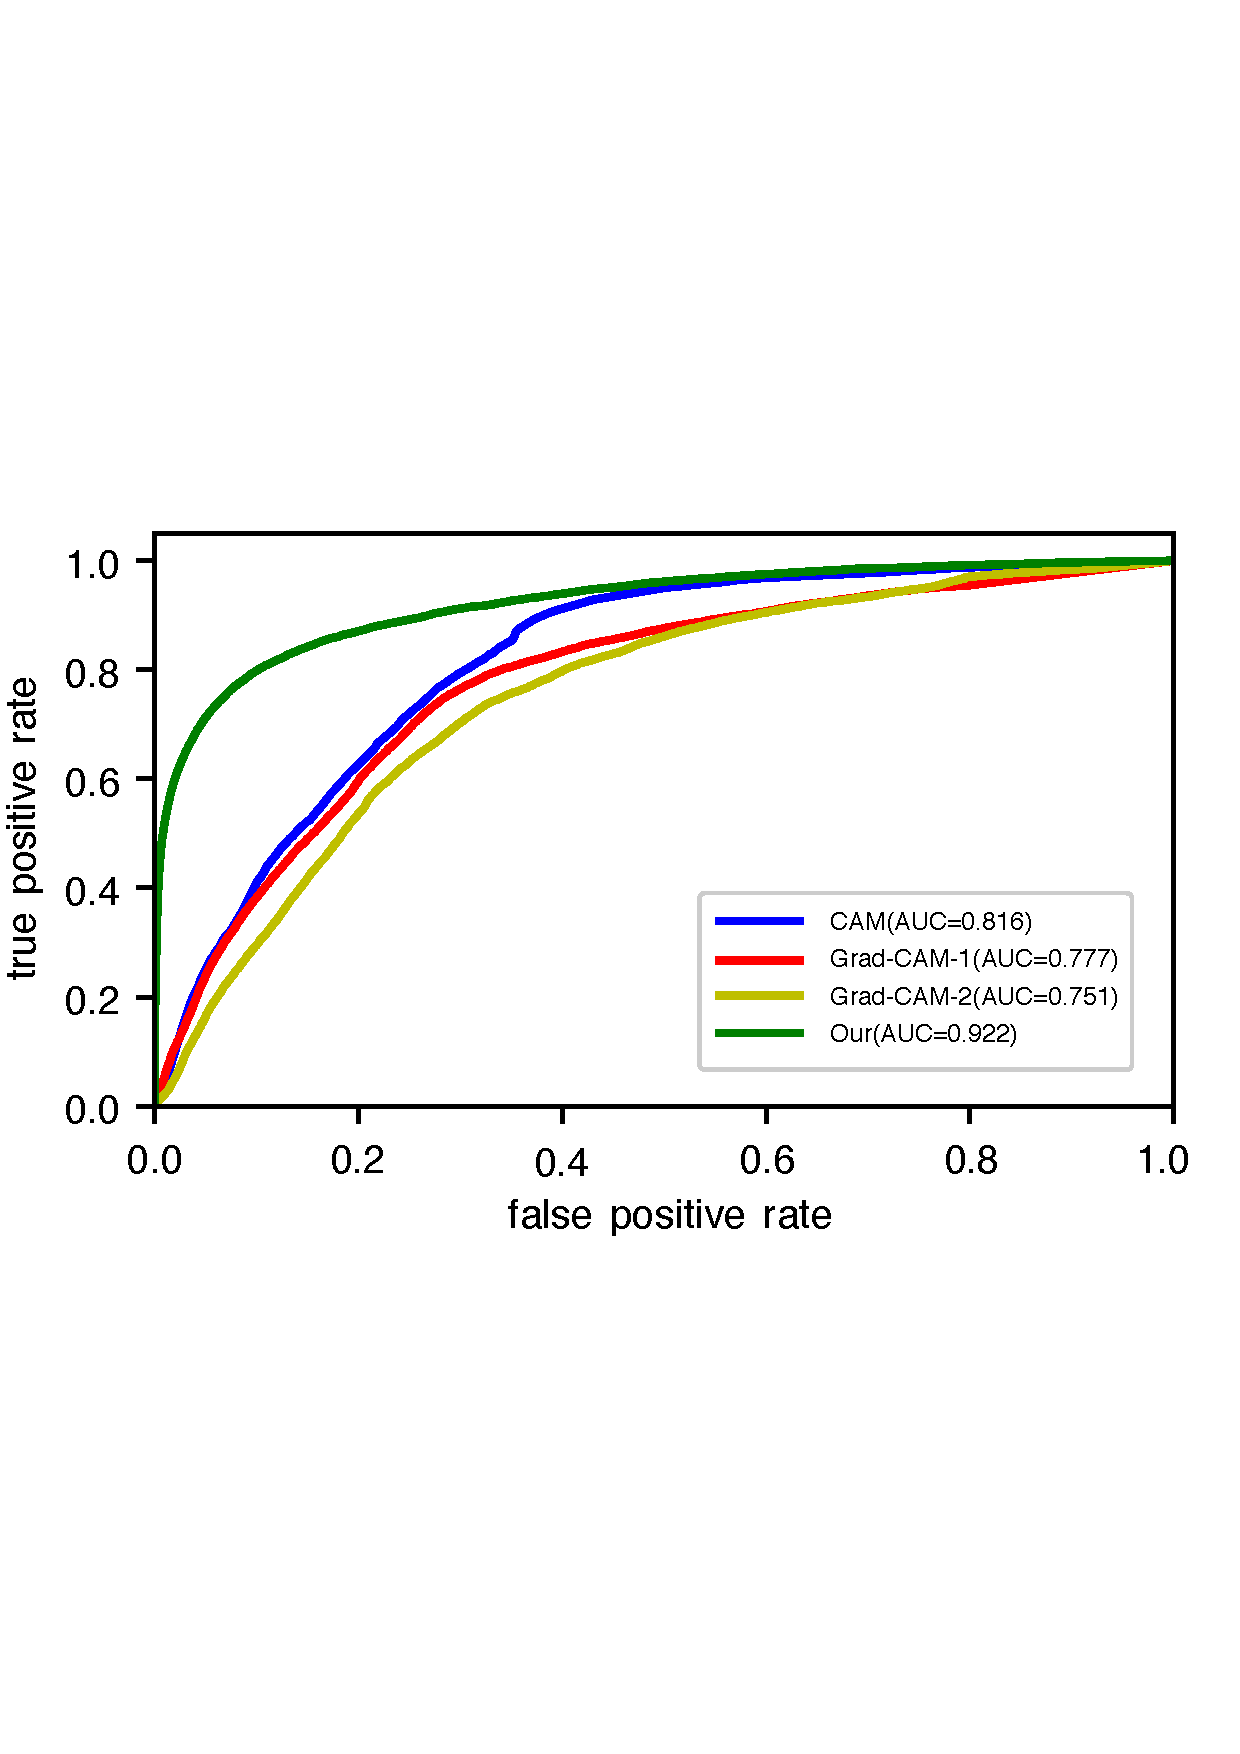
\includegraphics[width=1.0\textwidth]{figure/ROC_cam_grad_cam_our_diabetic_retinopathy}
	\caption{各种方法根据二类视网膜糖尿病病变数据集绘制的ROC曲线。ROC曲线是根据数据集中$40$张像素级标注图像绘制。在ROC曲线产生之前,先将各种方法的定位结果的热图归一化到$[0, 1]$。} 
	\label{fig:roc_cam_grad_cam_our_diabetic_retinopathy}
\end{figure}

从图\ref{fig:roc_cam_grad_cam_our_diabetic_retinopathy}可以看出,


\begin{figure}[h]
	\centering
	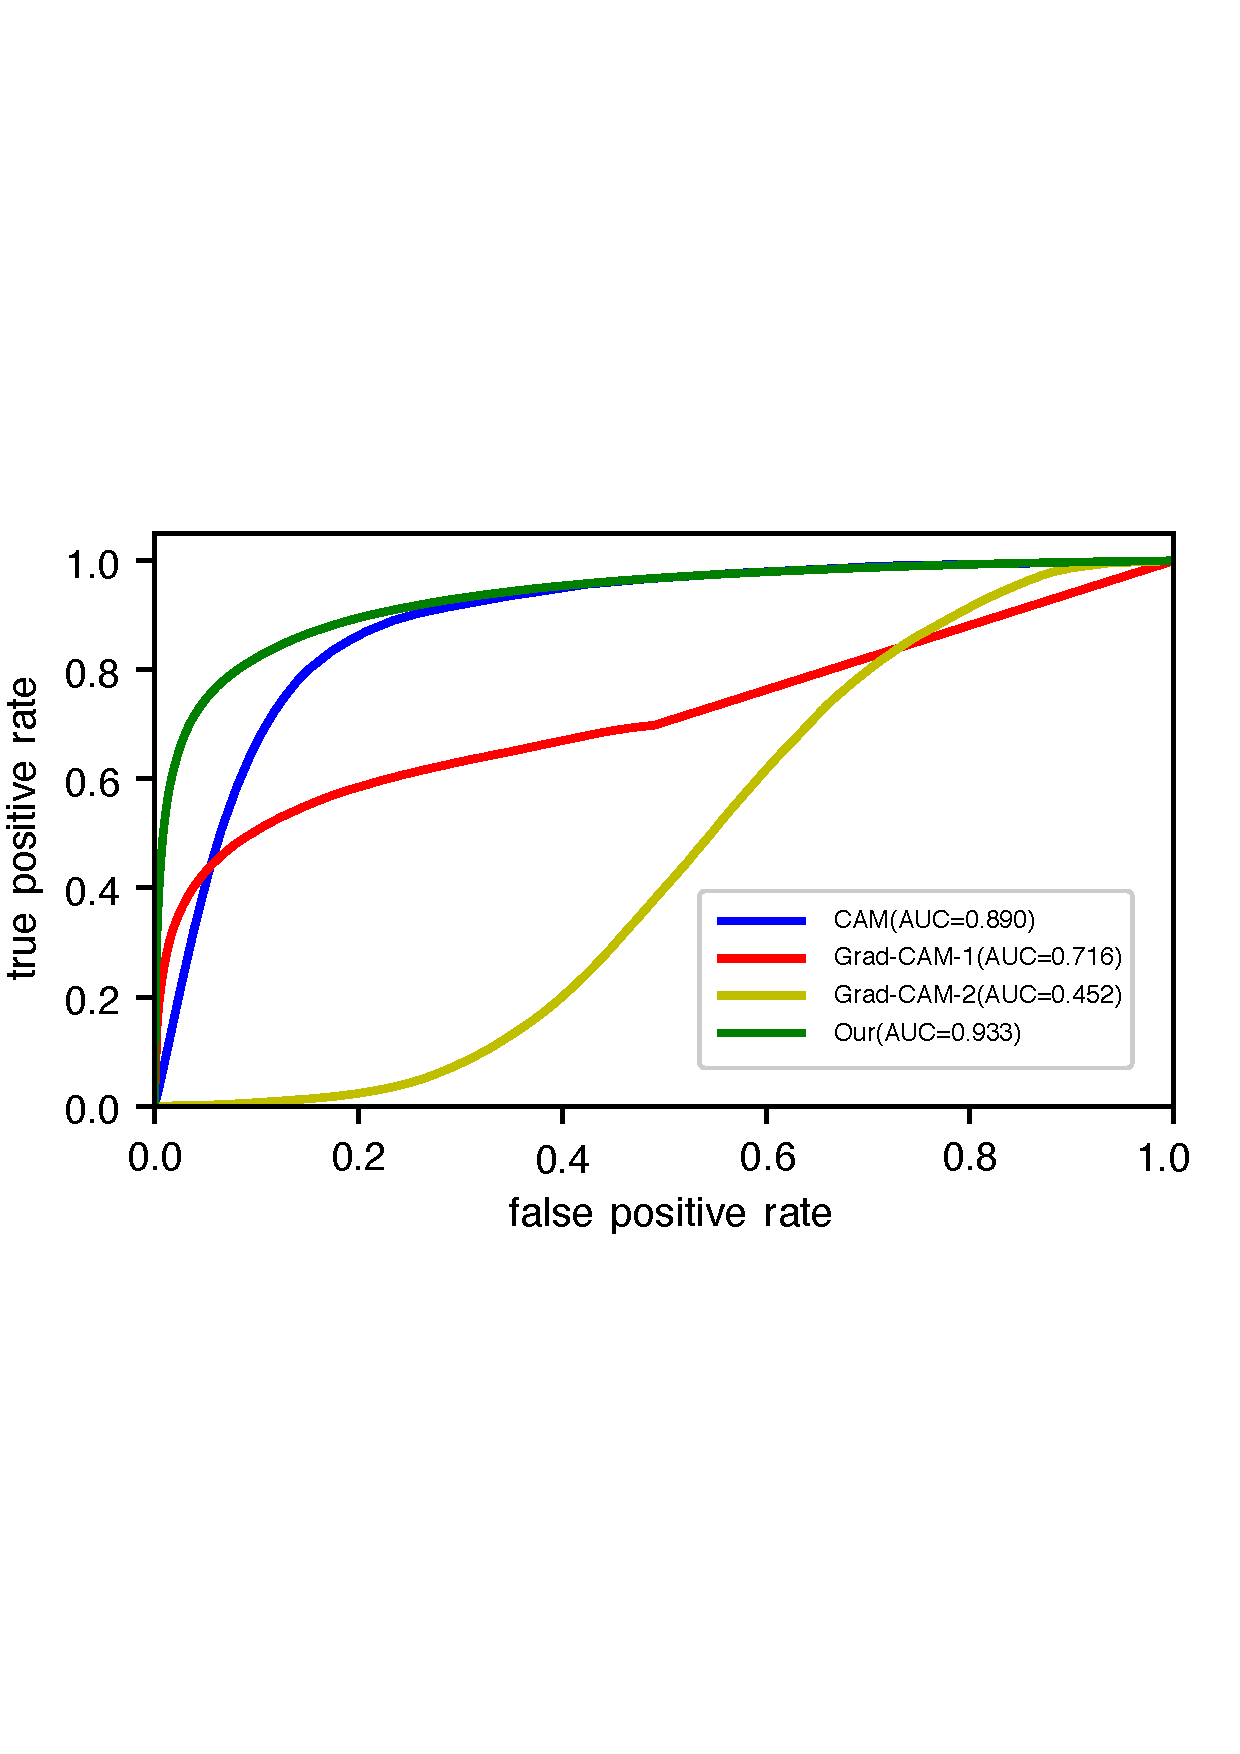
\includegraphics[width=1.0\textwidth]{figure/ROC_cam_grad_cam_our_simulated_skin_datasets}
	\caption{} 
	\label{fig:roc_cam_grad_cam_our_simulated_skin_datasets}
\end{figure}


\begin{figure}[h]
	\centering
	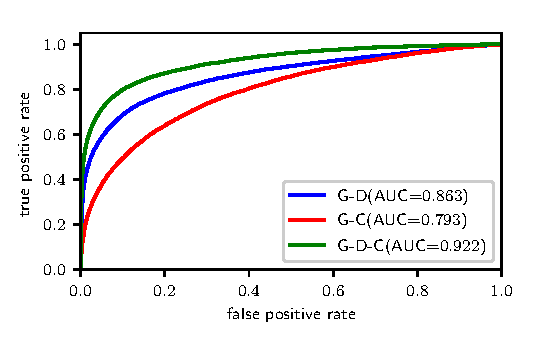
\includegraphics[width=1.0\textwidth]{figure/ROC_u_d_u_c_u_d_c_components}
	\caption{G-D模型、G-C模型和G-D-C模型根据二类视网膜糖尿病病变数据集中标注的部分图像绘制的P-R曲线。三条曲线各自对应的AUC见右上角图例。} 
	\label{fig:roc_u_d_u_c_u_d_c_components}
\end{figure}

\endinput
